\documentclass[10pt]{article}

\usepackage[margin=0.75in]{geometry}
\usepackage{amsmath,amsthm,amssymb,bm}
\usepackage{xcolor}
\usepackage{cancel}
\usepackage{graphicx}
\usepackage{changepage}
\usepackage{circuitikz}
\usepackage{pgfplots}
\usepackage{minted}
\usepackage{physics}
\usepackage{tikz}
\usepackage{tikz-3dplot}
\usepackage{hyperref}
\usepackage{cleveref}
\usepackage{siunitx}
\usepackage{fontspec}
\usepackage{relsize}
\usepackage{subfig}
\usepackage{todonotes}
\usepackage{contour}
\usepackage{pgffor}
\usepackage{multicol, multirow, booktabs}
\usepackage[breakable]{tcolorbox}
\usepackage[inline]{enumitem}

\theoremstyle{definition}
\newtheorem{problem}{Problem}
\newtheorem{soln}{Solution}

\pgfplotsset{compat=newest}
\usetikzlibrary{lindenmayersystems}
\usetikzlibrary{arrows}
\usetikzlibrary{calc}
\usetikzlibrary{positioning, fit}
\usetikzlibrary{3d, perspective}
\usetikzlibrary{math}
\usetikzlibrary{fadings}
\usetikzlibrary{angles,quotes} 
\usetikzlibrary{decorations.markings}

\definecolor{incolor}{HTML}{303F9F}
\definecolor{outcolor}{HTML}{D84315}
\definecolor{cellborder}{HTML}{CFCFCF}
\definecolor{cellbackground}{HTML}{F7F7F7}
\newcommand{\ui}{\hat{i}}
\newcommand{\uj}{\hat{j}}
\newcommand{\uk}{\hat{k}}
\newcommand{\ux}{\hat{\mathbf{x}}}
\newcommand{\uy}{\hat{\mathbf{y}}}
\newcommand{\uz}{\hat{\mathbf{z}}}
\newcommand{\uv}[1]{\hat{\bv{{#1}}}}
\newcommand{\pr}[1]{{#1^\prime}}
\newcommand{\pd}[2][]{{\frac{\partial^{#1}}{\partial {{#2}^{#1}}}}}
\newcommand{\dif}[2][]{{\frac{d^{#1}}{d{{#2}^{#1}}}}}
\newcommand{\grd}{\nabla}

\pgfdeclarelayer{background}  
\pgfsetlayers{background,main}
\AtBeginDocument{\RenewCommandCopy\qty\SI}

\makeatletter
\newcommand{\boxspacing}{\kern\kvtcb@left@rule\kern\kvtcb@boxsep}
\makeatother
\newcommand{\prompt}[4]{
    \ttfamily\llap{{\color{#2}[#3]:\hspace{3pt}#4}}\vspace{-\baselineskip}
}

\newcommand{\thevenin}[2]{
  \begin{center}
    \begin{circuitikz} \draw
      (0,0) -- (2,0) to[battery1, l_=$V_{Th}\eq#1$] (2,2) 
      to[resistor, l_=$R_{Th}\eq#2$] (0,2)
      ;
      \draw [o-] (-.07,2.079);
      \draw [o-] (-.07,0.079);
    \end{circuitikz}
  \end{center}
}

\newcommand{\norton}[2]{
  \begin{center}
    \begin{circuitikz} \draw
      (0,0) -- (3,0) to[american current source, l_=$I_{N}\eq#1$] (3,2) -- (0,2) (2,0)
      to[resistor, l=$R_{N}\eq#2$] (2,2)
      ;
      \draw [o-] (-.07,2.079);
      \draw [o-] (-.07,0.079);
    \end{circuitikz}
  \end{center}
}

\DeclareMathOperator{\Div}{div}
\DeclareMathOperator{\Curl}{curl}
\DeclareMathOperator{\sgn}{sgn}

\newcommand{\highlight}[1]{\colorbox{yellow}{$\displaystyle #1$}}
\newcommand{\ti}[1]{\widetilde{#1}}
\renewcommand{\div}[1]{\bv{\nabla}\cdot #1}
\renewcommand{\curl}[1]{\bv{\nabla}\times #1}

\newfontface{\Kaufmann}{Kaufmann}
\DeclareTextFontCommand{\kf}{\Kaufmann}
\newcommand{\scriptr}{\fontsize{12pt}{12pt}\kf{r}\fontsize{10pt}{10pt}}

\newfontface{\KaufmannB}{Kaufmann Bold}
\DeclareTextFontCommand{\kfb}{\KaufmannB}
\newcommand{\bscriptr}{\fontsize{12pt}{12pt}\kfb{r}\fontsize{10pt}{10pt}}
\newcommand{\justif}[2]{&{#1}&\text{#2}}
\newcommand{\bv}[1]{\bm{\mathrm{#1}}}

\title{Physics 4140H: Assignment I}
\author{Jeremy Favro (0805980) \\ Trent University, Peterborough, ON, Canada}
\date{\today}

\begin{document}
\maketitle

% PROBLEM 1
\begin{problem}~
\begin{enumerate}[label=(\alph*)]
  \item Find the curves on which the functional $$\int_{0}^{1}(y')^2+12xydx$$
        with $y(0)=0$ and $y(1)=1$ can be extremized.
  \item On which curve can the function $$\int_{0}^{\pi/2}(y')^2-y^2+2xydx$$
        with $y(0)=y(\pi/2)=0$ be extremized?
  \item Find the extrema of $$\int_{x_1}^{x_2}(1+x^2y')y'dx.$$
\end{enumerate}
\end{problem}
\begin{soln}~
  \begin{enumerate}[label=(\alph*)]
    \item Solving the Euler-Lagrange equation for $f(x)=(y')^2+12xy$,
          $$\frac{\partial f}{\partial y}=\frac{d}{dx}\left(\frac{\partial f}{\partial y'}\right).$$
          Here we have
          $$\frac{\partial f}{\partial y}=12x;\qquad \frac{\partial f}{\partial y'}=2y';\qquad \frac{d}{dx}\left(\frac{\partial f}{\partial y'}\right)=2y''.$$
          Hence we say that
          $$6x=y''$$ and integrate twice to obtain
          $$y=x^3+Cx+D$$
          and $y(0)=D=0$ and $y(1)=1+C=1\implies C=0$ so
          $$y(x)=x^3$$
    \item Again we apply the Euler-Lagrange equation with $f=(y')^2-y^2+2xy$ and obtain
          $$\frac{\partial f}{\partial y}=2x-2y;\qquad \frac{\partial f}{\partial y'}=2y';\qquad \frac{d}{dx}\left(\frac{\partial f}{\partial y'}\right)=2y''.$$
          So we say that
          $$x=y''+y.$$
          First we solve the homogenous form $y''+y=0$ by guessing a solution of the form $e^{mx}$ which gives a characteristic equation $m^2+1=0\implies m=i$
          and so we obtain $y_h=Ce^{ix}=C\cos(x)+C_1\sin(x)$. Then we solve for the particular solution by guessing at the method of undetermined coefficients with
          $y_p=x$ (which works). Hence the full solution is $y=C\cos(x)+C_1\sin(x)+x$. Applying the boundary conditions, $y(0)=C=0$ and $y(\pi/2)=C_2+\pi/2=0\implies C_2=-\pi/2$ hence
          $$y(x)=x-\frac{\pi}{2}\sin(x)$$
    \item Here
          $$\frac{\partial f}{\partial y}=0;\qquad \frac{\partial f}{\partial y'}=1+2x^2(y');\qquad \frac{d}{dx}\left(\frac{\partial f}{\partial y'}\right)=4x(y')+2x^2(y'').$$
          Hence
          $$2xy'+x^2y''=0$$
          which is a homogenous Cauchy-Euler equation and hence we take the solution to be of the form $y=x^m$ and obtain the characteristic equation
          $m^2+2m=0\implies m=0,-2$. Hence $y=C_1+C_2x^{-2}$.
  \end{enumerate}
\end{soln}

% PROBLEM 2
\begin{problem}~
\begin{enumerate}[label=(\alph*)]
  \item Review the brachistochrone problem (Example 6.2). Show that the time required for a
        particle to move (frictionless) to the minimum point of the cycloid is $\pi\sqrt{a/g}$ where ``a'' is as
        shown in the figure 6-4 and ``g'' is acceleration due to gravity. (Hint: Use your knowledge
        of equations of a cycloid from Example 6.2; set up the problem using the time from
        kinematic equations; just before minimization convert $x$ and $y$ in terms of $\theta$, using the
        equations of a cycloid).
  \item Plot the brachistochrone path in a Euclidian plane for $\theta$ varying from $0$ to $8\pi$.
\end{enumerate}
\end{problem}
\begin{soln}~
  \begin{enumerate}[label=(\alph*)]
    \item The integral we constructed to give the time taken on the shortest path (which we then minimized) was
          $$t=\int_{x_1}^{x_2}\sqrt{\frac{1+(y')^2}{2gx}}dx.$$
          In minimizing the time we found that $y=a(\theta-\sin\theta)$ and $x=a(1-\cos\theta)$ for constant $a$. We need to change the integral to
          one in terms of $\theta$ before we can plug in these results and calculate a time. To do this we recall from the minimization of $t$
          when we made a change of variable we found that $dx=a\sin(\theta)d\theta$ and then that
          $$y'=\frac{dy}{dx}=\frac{dy}{d\theta}\frac{d\theta}{dx}=\frac{1-\cos\theta}{\sin\theta}$$
          which we plug in to $t$ to obtain
          \begin{align*}
            t & =\int_{0}^{\theta_f}\sqrt{\frac{1+(\frac{1-\cos\theta}{\sin\theta})^2}{2ga(1-\cos\theta)}}a\sin(\theta)d\theta                                                       \\
              & =\frac{a}{\sqrt{2ga}}\int_{0}^{\theta_f}\sqrt{\frac{1+\frac{(1-\cos\theta)^2}{\sin^2\theta}}{(1-\cos\theta)}}\sin(\theta)d\theta                                     \\
              & =\sqrt{\frac{a}{2g}}\int_{0}^{\theta_f}\sqrt{\frac{\sin^2(\theta)+(1-\cos\theta)^2}{(1-\cos\theta)}}d\theta                                                          \\
              & =\sqrt{\frac{a}{2g}}\int_{0}^{\theta_f}\sqrt{\frac{\sin^2(\theta)+1-2\cos\theta+\cos^2(\theta)}{(1-\cos\theta)}}d\theta                                              \\
              & =\sqrt{\frac{a}{2g}}\int_{0}^{\theta_f}\sqrt{\frac{2(1-\cos\theta)}{(1-\cos\theta)}}d\theta=\sqrt{\frac{a}{g}}\int_{0}^{\theta_f}d\theta=\theta_f\sqrt{\frac{a}{g}}.
          \end{align*}
          $\theta_f$ will be $\pi$ since that is the maximum (since we flipped the $y$-direction) of the cycloid, or the minimum point that the ball reaches.
    \item Note that the plot appears flipped vertically from what we would expect because of our choice of axis in solving the original problem,
          the ball traveling along the brachistochrone path would be falling in the $+y$-direction.
          ~\begin{center}
            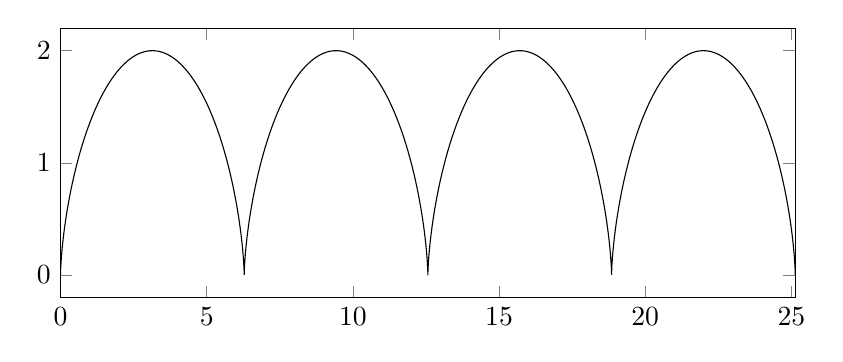
\begin{tikzpicture}
              \begin{axis}[
                  width=\textwidth*0.9, height = 5cm,
                  xmin=0, xmax=8*3.14159
                ]
                \def\a{1}
                \addplot[domain=0:8*3.14159, samples=400, color=black] ({(\a)*(\x-sin(deg(\x)))},{\a*(1-cos(deg(\x)))});
              \end{axis}
            \end{tikzpicture}
          \end{center}
  \end{enumerate}
\end{soln}

% PROBLEM 3
\begin{problem}
Fermat's Principle: Consider light passing from one medium with index of refraction $n_1$ into
another medium with index of refraction $n_2$. Use Fermat's principle and calculus of variation to
minimize time and derive the Snell's law of refraction: $n_1\sin\theta_1=n_2\sin\theta_2$. Geometry based
answers will receive zero points and are not accepted.
\end{problem}
\begin{soln}
  The total time required to move a distance is given by the integral
  $$t=\int_{x_1}^{x_2}\frac{ds}{v}.$$
  In non-absorbing media, light travels at a speed given by $c/n$ for (real) index of refraction $n$.
  As usual the light wants to travel a distance $ds=\sqrt{dx^2+dy^2}=\sqrt{1+(y')^2}dx$ transforming the integral to
  $$t=\int_{x_1}^{x_2}\frac{1}{v}\sqrt{1+(y')^2}dx=\int_{x_1}^{x_2}\frac{n}{c}\sqrt{1+(y')^2}dx.$$
  $n$ here is a function of $x$ as it changes between the media (I want to try to remember to ask a clarifying question
  about why we are allowed a discontinuous first derivative here). To minimize time taken then we apply the Euler-Lagrange equation
  with $f=\frac{n}{c}\sqrt{1+(y')^2}$. $\partial f/\partial y=0$, and
  $$\frac{\partial f}{\partial y'}=\frac{n}{c}\frac{y'}{\sqrt{1+(y')^2}}.$$
  Since $\partial f/\partial y=0$ we can say that
  $$\frac{\partial f}{\partial y'}=\frac{n}{c}\frac{y'}{\sqrt{1+(y')^2}}=A$$
  for constant $A$. Since $n$ is a step-function,
  $$A=\begin{cases}
      \frac{n_1}{c}\frac{y_1'}{\sqrt{1+(y_1')^2}} & x\in(x_1,x_m) \\
      \frac{n_2}{c}\frac{y_2'}{\sqrt{1+(y_2')^2}} & x\in(x_m,x_2)
    \end{cases}$$
  where $x_m$ represents the position of interface between the two media the light is traveling through, $y_1$ and $y_2$ the light paths in those media.
  Since both cases are equal to a constant, we can say that
  $$\frac{n_1}{c}\frac{y_1'}{\sqrt{1+(y_1')^2}}=\frac{n_2}{c}\frac{y_2'}{\sqrt{1+(y_2')^2}}.$$
  Rewriting the derivatives
  $$n_1\frac{\frac{dy_1}{dx}}{\sqrt{1+(\frac{dy_1}{dx})^2}}=n_2\frac{\frac{dy_2}{dx}}{\sqrt{1+(\frac{dy_2}{dx})^2}}$$
  and multiplying through by $\frac{dx}{dx}$
  $$n_1\frac{dy_1}{\sqrt{(dx)^2+(dy_1)^2}}=n_2\frac{dy_2}{\sqrt{(dx)^2+(dy_2)^2}}.$$
  We then have to make the geometric realization that $\sin(\theta)$ is opposite/hypotenuse, and for the triangle of sides
  $dx$ and $dy$, $\sin\theta=\frac{dy}{\sqrt{(dx)^2+(dy)^2}}$
  so
  $$n_1\sin\theta_1=n_2\sin\theta_2.$$
\end{soln}


% PROBLEM 4
\begin{problem}
Find the shortest path between two points $(x_1, y_1, z_1)$ and $(x_2, y_2, z_2)$ in a 3-dimensional
Euclidean space.
\end{problem}
\begin{soln}
Skipping the steps of setup because we clearly want to minimize the arc-length,
we obtain three differential equations involving $f=\sqrt{1+(y_i')^2}$,
$$\frac{\partial f}{\partial y_i}=\frac{d}{dx}\left(\frac{\partial f}{\partial y_i'}\right),\quad i=1,2,3.$$
Each of these will have the same solution since 
$$\frac{\partial f}{\partial y_i'}=\frac{y_i'}{\sqrt{1+(y_i')^2}}=C\forall i$$
which gives a solution 
$$y_i=C_1x_i+C_2.$$
Hence, minimizing the per-component integrals from $(x_1, y_1, z_1)$ to $(x_2, y_2, z_2)$ yields equations for three lines,
which form the equation for a line between two arbitrary points in $\mathbb{R}^3$.
\end{soln}

% PROBLEM 5
\begin{problem}~
\begin{enumerate}[label=(\alph*)]
  \item Learn Example 6.1. Plot the neighbouring function using the definition given in the book:
        $\eta(x)$, $y(x)$, and $y(\alpha,x)$ within the specified limit. Finally obtain $J(\alpha)$ and argue that it
        must be higher than extremum value of $J$.
  \item Compare a catenary path and a parabolic path by plotting them in the same graph.
\end{enumerate}
\end{problem}
\begin{soln}~
  \begin{enumerate}[label=(\alph*)]
    \item In Example 6.1, $y(x)=x$, $\eta(x)=\sin(x)$ and hence $y(\alpha,x)=x+\alpha\sin(x)$. Plotting this we obtain
          ~\begin{center}
            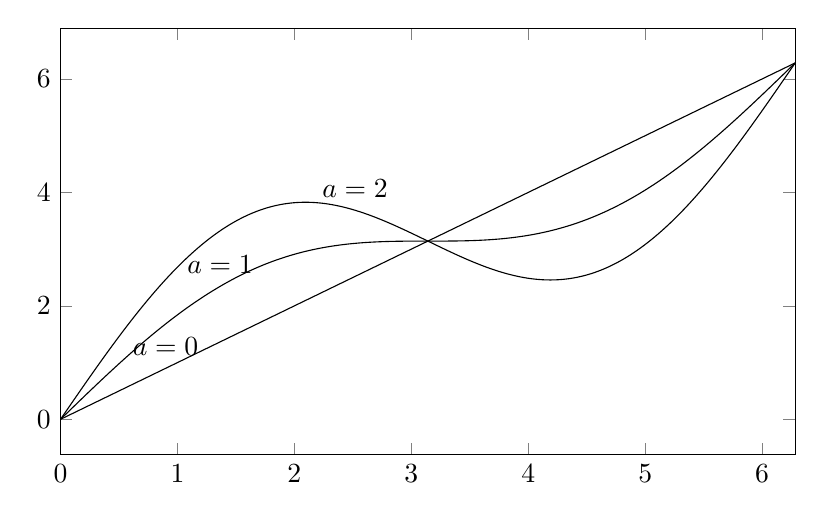
\begin{tikzpicture}
              \begin{axis}[
                  width=\textwidth*0.9, height = 7cm,
                  xmin=0, xmax=2*3.14159
                ]
                \pgfplotsinvokeforeach {0,1,2}{
                  \addplot[domain=0:3.14159*2, samples=400, color=black] (\x,{\x+#1*sin(deg(\x))}) node[pos=(#1+1)/7, above, yshift=1.1]{$a=#1$};
                }
              \end{axis}
            \end{tikzpicture}
          \end{center}
          This gives
          $$J(\alpha)=\int_0^{2\pi} (y')^2dx=\int_0^{2\pi} \left[1+\alpha\cos(x)\right]^2dx=\int_0^{2\pi} 1+2\alpha\cos(x)+\alpha^2\cos^2(x)dx=2\pi+\alpha^2\pi$$
          where I've chosen the bounds of integration to include a full period. No matter what $\alpha\neq 0$ it will be greater than $J(0)$ (the extremum value),
          since $\alpha^2>0$. Hence $y(0,x)$ is the shortest path, and $J(0)$ is an extremum.
    \item ~\begin{center}
            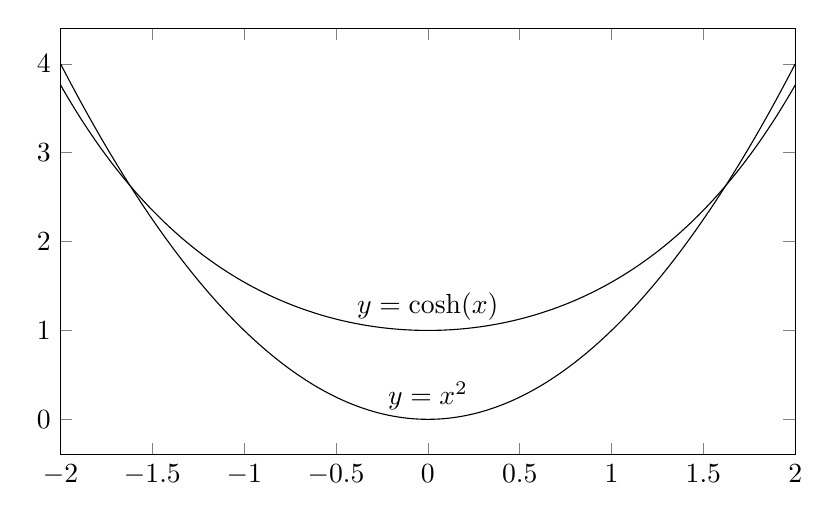
\begin{tikzpicture}
              \begin{axis}[
                  width=\textwidth*0.9, height = 7cm,
                  xmin=-2, xmax=2
                ]
                \addplot[domain=-2:2, samples=400, color=black] (\x,{\x^2}) node[midway, above]{$y=x^2$};
                \addplot[domain=-2:2, samples=400, color=black] (\x,{cosh(\x)}) node[midway, above]{$y=\cosh(x)$};
              \end{axis}
            \end{tikzpicture}
          \end{center}
          The catenary ($\cosh(x)$) has smaller absolute slope and is ``wider'' as a result. Obviously to traverse the distance between their intersections,
          the catenary is a shorter path.
  \end{enumerate}
\end{soln}
\end{document}